\documentclass{article}
\usepackage[T1]{fontenc}
\usepackage{lmodern}
\usepackage{graphicx}
\usepackage{amsmath,amssymb}
\usepackage[a4paper,margin=2cm]{geometry}
\usepackage[absolute,overlay]{textpos}
\setlength{\TPHorizModule}{1mm}
\setlength{\TPVertModule}{1mm}
\usepackage[indonesian]{babel}
\usepackage{hyperref}
\setlength{\emergencystretch}{2em}
% unit: Halaman 47

\begin{document}

% === Halaman 47 (llm) ===

Sumber: William Stalling, Cryptography and Network Security
Overview \& Chapter 1

\vspace{60mm}

\begin{center}
\textbf{\huge Active Attack: Replay}
\end{center}

% deskripsi: Ilustrasi serangan replay yang melibatkan Bob sebagai pengirim, Alice sebagai penerima, dan Darth sebagai penyerang yang menangkap serta mengirim ulang pesan melalui jaringan internet.
% bbox normalisasi: [0.1780, 0.2180, 0.8220, 0.7900]
\begin{textblock*}{135.24mm}(37.38mm,64.75mm)
\noindent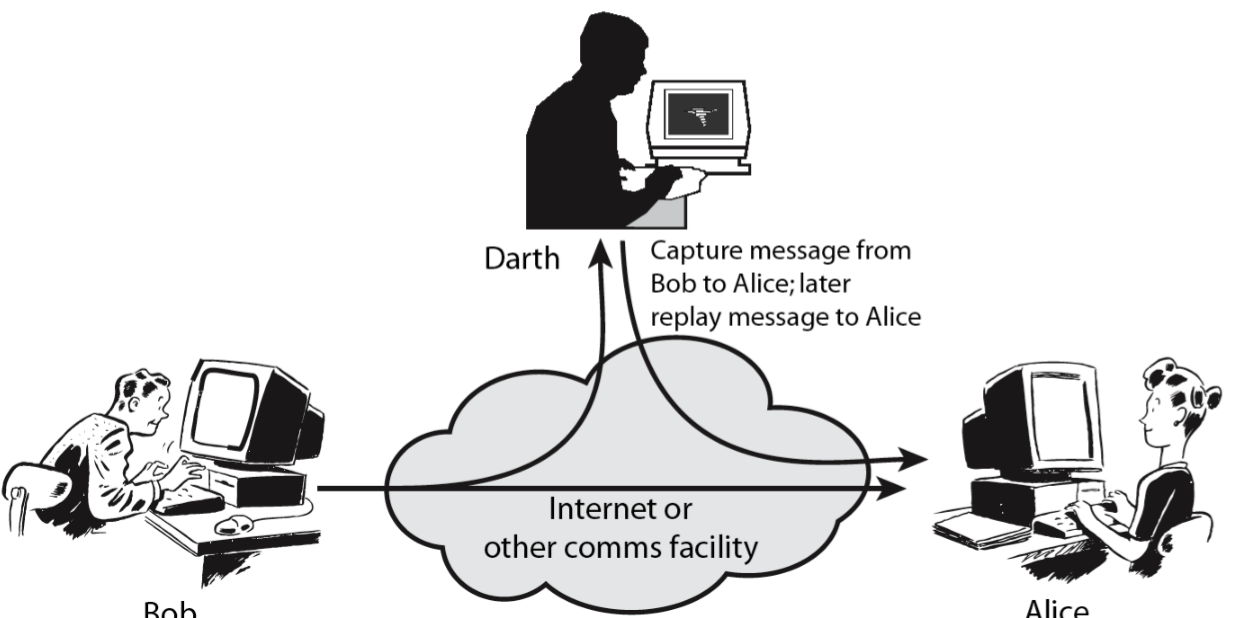
\includegraphics[width=135.24mm,height=169.88mm]{../../images/llm/page_047_img_01.png}%
\end{textblock*}

\end{document}
